% siminos/presentations/Lisbon21/Lisbon21.tex  pdflatex Lisbon21; biber Lisbon21
% $Author: predrag $ $Date: 2021-12-07 18:54:06 -0500 (Tue, 07 Dec 2021) $

% FROZEN                                            \date{December 6, 2021}

%  started with siminos/presentations/Haake21/Haake21.tex   2020-12-16
%         and   siminos/presentations/kittens/*.tex
%  lectures/QFT20/ kittens.pdf saved as                     2020-09-27
%          ChaosBook.org/overheads/spatiotemporal/QFT20.pdf
%  started with siminos/presentations/GTmath18/GTmath18.tex 2018-03-02
%  started with siminos/presentations/KITP17/UCSB17.tex     2017-01-26
%  started with siminos/presentations/Israel16/Israel16.tex 2016-08-17
%  started with siminos/presentations/GTmap16/GTmap16.tex   2016-08-17
%  started with talks/predrag/NBI16/NBI16.tex               2016-04-25
%  started with talks/predrag/RoySoc16/RoySoc16.tex         2016-04-25

                        \newif\ifboyscout\boyscouttrue          %% comments     %%
                        \newif\ifsubmission\submissionfalse     %% internal     %%
                        \newif\ifblog\blogfalse %% section shared with blogCats %%

\input ../../inputs/layoutBeamer
\usepackage[font=scriptsize, labelfont=bf]{caption}
\usepackage[
    backend=biber,  %bibtex,
    sorting=nyt,
    %refsection=chapter,
    %citereset=chapter,
    style=numeric, %alphabetic, % %style=authoryear,
    natbib=true,
    style=phys, % aps
    biblabel= brackets, % superscript, %
    articletitle=false, % true,  % false, % aps
    %chaptertitle=true,  % aip;  % false, % aps
    pageranges = true , % aip: the full range
             % = false, % aps: only the first page being printed
    sortlocale=en_US,
    firstinits=true,
    url=false, %true,  %
    doi=false, %true,
    eprint=false
]{biblatex}
\addbibresource{../../bibtex/siminos.bib}
\setbeamerfont{footnote}{size=\tiny}
%\input ../../inputs/def % no edits, always from dasbuch/book/inputs
\input ../kittens/defsKittens
\input ../../inputs/defsBeamer
\renewcommand{\Ssym}[1]{{\ensuremath{m_{#1}}}}    % Boris

\begin{document}
\title{
{\huge herding cats} %\catlatt}
    \\
{a chaotic field theory}
}
\author{P. Cvitanovi\'c}
\author[Cvitanovi\'c]
{
  \textcolor{green!50!black}{
  {Predrag~Cvitanovi\'c
   and
   Han Liang
%   \\
%  Matt Gudorf,
  }	%\inst{1}
  }
}
\institute
{
%               Georgia Tech
% \\
%  \inst{1}%
%\HREF{https://itsatcuny.org/calendar/chaos-and-quantum-field-theory}
%{ITS Symposium on Chaos and Quantum Field Theory}
    {\scriptsize
\HREF{https://ChaosBook.org/overheads/spatiotemporal}
 {ChaosBook.org/overheads/spatiotemporal}
 \\ $\to$ Chaotic field theory slides
 \\ $\to$ \HREF{https://educast.fccn.pt/vod/channels/1x4mvd1fjn}
   {$QM^3$ video channel}
    }
 \\ \bigskip
\HREF{https://qm3.tecnico.ulisboa.pt/seminars?id=6461}
    {"$QM^3$ Quantum Matter meets Maths"}
 \\
                Lisbon
 }
\date{December 6, 2021}

\renewcommand{\Refl}{\ensuremath{\sigma}}             % in DasBuch
\renewcommand{\ssp}{\ensuremath{\phi}}             % lattice site field
\renewcommand{\Xx}{\ensuremath{\Phi}}
% \renewcommand{\Xx}{\ensuremath{\mathsf{\Phi}}}      % kittens lattice field
\renewcommand{\Ssym}[1]{{\ensuremath{m_{#1}}}}    % Boris


\begin{frame}
  \titlepage
\end{frame} %%%%%%%%%%%%%%%%%%%%%%%%%%%%%%%%%%%%%%%%%%%%%%

\begin{frame}{} %herding cats}
\begin{center}
\hfill\includegraphics[width=0.95\textheight]{DawnBishopCats}
\end{center}
\end{frame} %%%%%%%%%%%%%%%%%%%%%%%%%%%%%%%%%%%%%%%%%%%%%%

%%%%%%%%%%%%%%%%%%%%%%%%%%%%%%%%%%%%%%%%%%%%%%%%%%%%%%%%%%%%%%%%%%%%%%%%
\begin{frame}{Q. what is a chaotic field theory?}
    \begin{block}{A. it is a field theory}
\textcolor{blue}{field configuration} \Xx\ probability
\[
p(\Xx)\,=\, \frac{1}{Z}\,e^{-S[\Xx]}
\,,\qquad Z=Z[0]
\] % ee{ProbConf}
\textcolor{blue}{partition function} $=$ sum over configurations
\beq
Z[\source]	% = e^{W[\source]}
    \,=\, \int [d\ssp]\,e^{-S[\Xx] + \Xx \cdot \source}
    \,,\qquad
\left[ d\ssp\right] = \prod_{z}^{\lattice} \frac{d\ssp_z}{\sqrt{2 \pi}}
\label{n-pt-corr}
\eeq
    \end{block}
%\textcolor{blue}{`source'} $\source$
\bigskip

    \begin{block}{example : Euclidean {$\phi^4$} theory \textcolor{blue}{action}}
\bea
S[\Xx] &=& \int dx^d \left\{ \frac{1}{2} \sum_{i =1}^d
(\partial_{\mu}\ssp(x))^2 + \frac{\mu^2}{2}\ssp(x)^2 + \frac{g}{4!}\ssp(x)^4
\right\}
\eea
    \end{block}
\end{frame} %%%%%%%%%%%%%%%%%%%%%%%%%%%%%%%%%%%%%%%%%%%%%%

%%%%%%%%%%%%%%%%%%%%%%%%%%%%%%%%%%%%%%%%%%%%%%%%%%%%%%%%%%%%%%%%%%%%%%%%
\begin{frame}{Q. why a "chaotic" field theory?}
\vfill
\begin{center}
{\huge turbulence !}
\end{center}
\vfill
\end{frame} %%%%%%%%%%%%%%%%%%%%%%%%%%%%%%%%%%%%%%%%%%%%%%

\begin{frame}{a motivation : need a theory of {\Huge large} turbulent domains}
pipe flow close to onset of turbulence
\footnote{M.~Avila and B.~Hof, {Phys. Rev. \bf E 87} (2013)}
\begin{center}
\includegraphics[width=1.0\textwidth]{AviHof13fig4CLM}
\end{center}
we have a detailed theory of {\small \textcolor{blue}{small}} turbulent fluid cells

\bigskip

can we can we construct the \textcolor{red}{infinite} pipe by coupling small turbulent cells ?
\bigskip

\textcolor{blue}{what would that theory look like ?}
\end{frame} %%%%%%%%%%%%%%%%%%%%%%%%%%%%%%%%%%%%%%%%%%%%%%


\begin{frame}{the goal}
\vfill

\begin{center}
{\Large build
\\
a \textcolor{blue}{chaotic field theory}
\medskip

from
\\
the simplest \textcolor{blue}{chaotic blocks}
}
\end{center}

\vfill
using
\begin{itemize}
  \item
\textcolor{blue}{time invariance}
  \item
\textcolor{blue}{space invariance}
\end{itemize}
 of the defining partial differential equations
\end{frame} %%%%%%%%%%%%%%%%%%%%%%%%%%%%%%%%%%%%%%%%%%%%%%

\begin{frame}{Dreams of Grand Schemes : solve}
 \begin{center}
   \includegraphics[width=0.60\textwidth]{02-DreamEqs}
 \end{center}
\end{frame}

\begin{frame}{QFT path integrals : semi-classical WKB quantization}
  \begin{columns}
  \column{0.42\textwidth}
\begin{block}{a local unstable extremum}
\includegraphics[width=1.00\textwidth,clip=true]{saddle}%
\end{block}
  \column{0.50\textwidth}
\begin{block}{a fractal set of saddles}
\includegraphics[width=1.00\textwidth,clip=true]{pde2}%
\end{block}
  \end{columns}
\end{frame}

\begin{frame}{Q. what is a chaotic field theory?}
    \begin{block}{A. say it three times}
{\textcolor{blue}{coin flip}}
\bigskip

\hfill serves here as an introduction to the

{\textcolor{blue}{\catlatt}\footfullcite{CL18}}
\bigskip

\hfill which is the simplest example of % the larger picture

 \textcolor{blue}{spatiotemporally chaotic field theory}\footfullcite{GuBuCv17}
\bigskip\bigskip\bigskip
    \end{block}
\end{frame} %%%%%%%%%%%%%%%%%%%%%%%%%%%%%%%%%%%%%%%%%%%%%%

\begin{frame}{take-home :   }
\begin{center}
            \begin{minipage}[c]{0.40\textwidth}\begin{center}
{\color{purple}harmonic} field theory
\bigskip

\includegraphics[width=0.85\textwidth]{mattressSpring}\\
{\color{blue}tight-binding} model \\ ({\color{blue}Helmholtz})
            \end{center}\end{minipage}
            \hspace{2ex}
            \begin{minipage}[c]{0.46\textwidth}\begin{center}
{\color{purple}chaotic} field theory\\
\bigskip
\bigskip
\bigskip

\includegraphics[width=1.0\textwidth]{flagellum1}\\
\bigskip

Euclidean {\color{blue}Klein-Gordon} \\ (damped {\color{blue}Poisson})
            \end{center}\end{minipage}
\end{center}
\end{frame}%%%%%%%%%%%%%%%%%%%%%%%%%%%%%%%%%%%%%%%%%%%%%%

\begin{frame}{take-home :   }
\begin{center}
            \begin{minipage}[c]{0.40\textwidth}\begin{center}
{\color{purple}harmonic} field theory
\bigskip

\includegraphics[width=0.35\textheight]{twodlinearEll}\\
\bigskip

{\color{blue}oscillatory eigenmodes}
            \end{center}\end{minipage}
            \hspace{2ex}
            \begin{minipage}[c]{0.46\textwidth}\begin{center}
{\color{purple}chaotic} field theory\\
\bigskip

\includegraphics[width=0.35\textheight]{twodlinearHyp}\\
\bigskip

{\color{blue}hyperbolic instabilities}
            \end{center}\end{minipage}
\end{center}
\end{frame} %%%%%%%%%%%%%%%%%%%%%%%%%%%%%%%%%%%%%%%%%%%%%%


%%%%%%%%%%%%%%%%%%%%%%%%%%%%%%%%%%%%%%%%%%%%%%%%%%%%%%%%%%
\section[a coin toss]
 {a coin toss}

%%%%%%%%%%%%%%%%%%%%%%%%%%%%%%%%%%%%%%%%%%%%%%%%%%%%%%%%%%
\begin{frame}{}
\begin{bartlett}{
Mephistopheles knocks at Faust's door and says, ``Du
mu{\ss}t es dreimal sagen!"
\\{\color{yellow}.}\qquad
{\scriptsize\emph{``You have to say it three times"}}
        }
\bauthor{
Johann Wolfgang von Goethe
\\{\color{yellow}.}\qquad\quad
{\em Faust I - Studierzimmer 2.~Teil}%\rf{GoetheIstuZim1806}
    }
\end{bartlett}
\vfill
\begin{enumerate}
              \item \textcolor{gray}{\small
\HREF{http://ChaosBook.org/overheads/spatiotemporal/why.pdf}
{what this is about}
                    }
              \item {\Large
\HREF{http://ChaosBook.org/overheads/spatiotemporal/Bernoulli.pdf}
{coin toss}
                  }\textcolor{gray}{\small
              \item
\HREF{http://ChaosBook.org/overheads/spatiotemporal/templatt.pdf}
{\templatt}
              \item
\HREF{http://ChaosBook.org/overheads/spatiotemporal/catlatt.pdf}
{\catlatt}
              \item
\HREF{http://ChaosBook.org/overheads/spatiotemporal/timeDead.pdf}
{bye bye, dynamics}
                    }
            \end{enumerate}
\end{frame} %%%%%%%%%%%%%%%%%%%%%%%%%%%%%%%%%%%%%%%%%%%%%%

\renewcommand{\statesp}{state space}
\renewcommand{\ssp}{\ensuremath{x}}               % state space point

%%%%%%%%%%%%%%%%%%%%%%%%%%%%%%%%%%%%%%%%%%%%%%%%%%%%%%%%%%
\begin{frame}{(1)  coin toss, if you are stuck in XVIII century}
\vfill
    \begin{center}
{\huge time-evolution formulation}
    \end{center}
\vfill
\end{frame} %%%%%%%%%%%%%%%%%%%%%%%%%%%%%%%%%%%%%%%%%%%%%%

\begin{frame}{fair coin toss} % ~~~(AKA  }
\renewcommand{\ssp}{\ensuremath{\phi}}             % lattice site field
    \begin{block}{{Bernoulli}  map} %the essence of deterministic chaos}
\begin{center}
            \begin{minipage}[c]{0.36\textwidth}\begin{center}
% ChaosBook {fig:BernPartExam}
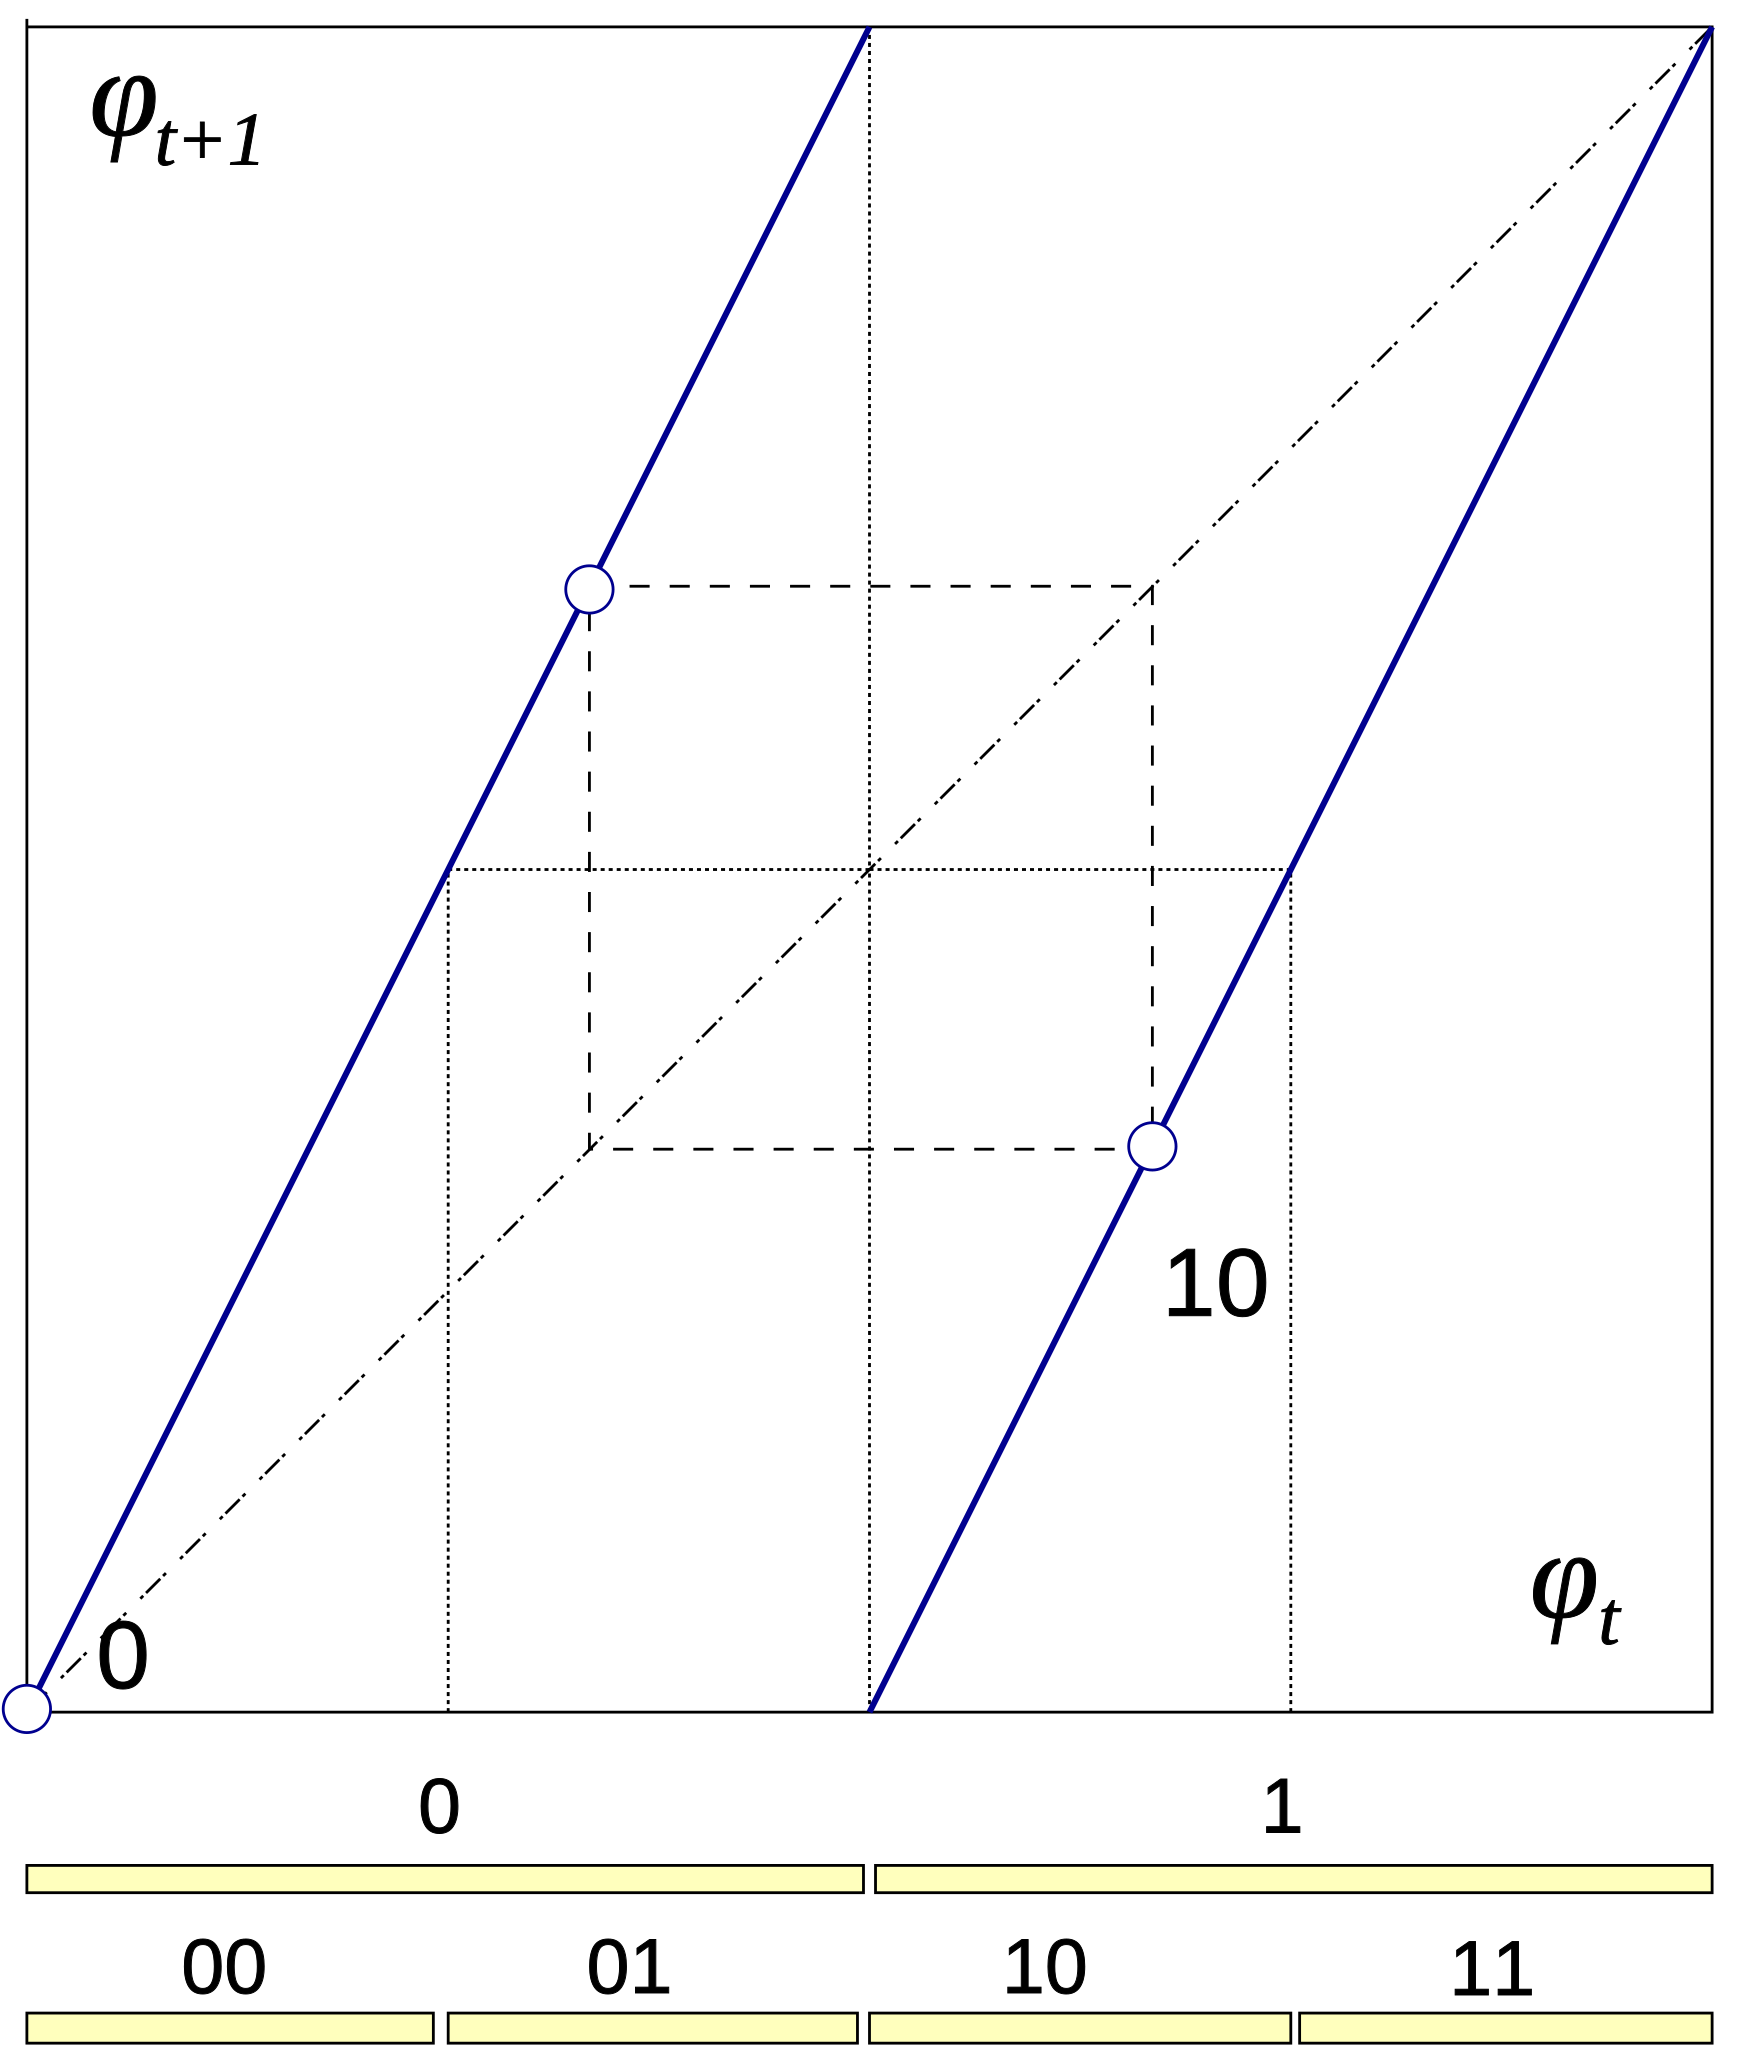
\includegraphics[width=1.0\textwidth]{BernPartKitten}
            \end{center}\end{minipage}
            \hspace{2ex}
            \begin{minipage}[c]{0.46\textwidth}\begin{center}
\[
\ssp_{\zeit+1} =
% \flow{}{\ssp_{\zeit}} =
\left\{ \begin{array}{l} %l}
        % f_0(\ssp_{\zeit}) =
        2 \ssp_{\zeit}
                             \\% \,, \quad & \ssp_{\zeit} \in \pS_0=[0,1/2) \\
        % f_1(\ssp_{\zeit}) =
        2 \ssp_{\zeit} \;\; (\mbox{mod}\;1)
                             % \,, \quad       & \ssp_{\zeit} \in \pS_1 =[1/2,1)
         \end{array}\right.
\]
            \end{center}\end{minipage}
\end{center}
%$\cl{}=2$ and 4 intervals \statesp\ partitions,

\hfill $\Rightarrow$~~~~~
fixed point \cycle{0}, 2-cycle \cycle{01}, $\cdots$
    \end{block}

\bigskip

a \HREF{https://www.random.org/coins/?num=2&cur=40-antique.aurelian}
{coin toss}

\hfill the essence of {\color{blue}deterministic chaos}
\end{frame} %%%%%%%%%%%%%%%%%%%%%%%%%%%%%%%%%%%%%%%%%%%%%%

\begin{frame}{what is ({mod}\;1) ?}
\renewcommand{\ssp}{\ensuremath{x}}             % lattice site field
map with integer-valued {\color{blue}`stretching' parameter $s\geq2$} :
\[
\ssp_{\zeit+1} \,=\, {s}\,\ssp_{\zeit}
\] %ee{BerStretch}

$(\mbox{mod}\;1)$ :
subtract the integer part
\(
\Ssym{\zeit}=\left\lfloor{s}\ssp_{\zeit}\right\rfloor
\)

\renewcommand{\ssp}{\ensuremath{\phi}}             % lattice site field
so fractional part
$\ssp_{\zeit+1}$ stays in the unit interval $[0,1)$
\[
\ssp_{\zeit+1} = {s} \ssp_{\zeit} - \Ssym{\zeit}
\,,\qquad  \ssp_{\zeit}\in\pS_{\Ssym{\zeit}}
\] %ee{circ-m}
$\Ssym{\zeit}$ takes values in the ${s}$-letter alphabet
\[
\Ssym{} \in \A=\{0,1,2,\cdots,s-1\}
\] %ee{base-sAlph}
\end{frame} %%%%%%%%%%%%%%%%%%%%%%%%%%%%%%%%%%%%%%%%%%%%%%

\renewcommand{\ssp}{\ensuremath{\phi}}             % lattice site field
% \renewcommand{\Xx}{\ensuremath{\mathsf{\Phi}}}      % kittens lattice field
\renewcommand{\ssp}{\ensuremath{\phi}}             % lattice site field
% \renewcommand{\Xx}{\ensuremath{\mathsf{\Phi}}}      % kittens lattice field
\begin{frame}{a fair dice throw}
    \begin{block}{slope ${6}$ Bernoulli map}
\begin{center}
            \begin{minipage}[c]{0.32\textwidth}\begin{center}
% ChaosBook {fig:BernPartExam}
\includegraphics[width=1.0\textwidth]{fig_d_2kitten} % {fig_d_2CL18}
            \end{center}\end{minipage}
            \hspace{2ex}
            \begin{minipage}[c]{0.46\textwidth}
\(
\ssp_{\zeit+1}
= {6} \ssp_{\zeit} - \Ssym{\zeit}
\,,\;  \ssp_{\zeit}\in\pS_{\Ssym{\zeit}}
\)
\medskip

${6}$-letter alphabet \\
\(
\Ssym{\zeit} \in \A=\{0,1,2,\cdots,5\}
\)
            \end{minipage}
\end{center}
$6$ subintervals $\{\pS_{0},\pS_{1},\cdots,\pS_{5}\}$
    \end{block}
\end{frame} %%%%%%%%%%%%%%%%%%%%%%%%%%%%%%%%%%%%%%%%%%%%%%

\begin{frame}{what is chaos ?}
    \begin{block}{a fair dice throw}
$6$ subintervals $\{\pS_{\Ssym{\zeit}}\}$,
$6^2$ subintervals $\{\pS_{\Ssym{1}\Ssym{2}}\}, \cdots$
\begin{center}
            \begin{minipage}[c]{0.32\textwidth}\begin{center}
% ChaosBook {fig:BernPartExam}
\includegraphics[width=1.0\textwidth]{fig_d_2kitten} % {fig_d_2CL18}
            \end{center}\end{minipage}
            \hspace{2ex}
            \begin{minipage}[c]{0.46\textwidth}
each subinterval contains a periodic point,
labeled by
$\Mm=\Ssym{1}\Ssym{2}\cdots\Ssym{\cl{}}$
\bigskip

$N_\cl{} = 6^\cl{}-1$ {\color{red}unstable} orbits
            \end{minipage}
\end{center}
    \end{block}
\vfill
    \begin{block}{definition : chaos is}
positive Lyapunov $(\ln s)$ - positive entropy $(\frac{1}{\cl{}}\ln N_\cl{})$
    \end{block}
\end{frame} %%%%%%%%%%%%%%%%%%%%%%%%%%%%%%%%%%%%%%%%%%%%%%

\begin{frame}{}
    \begin{block}{definition : chaos is}
positive {\color{blue}Lyapunov} $(\ln s)$
         -
positive {\color{blue}entropy} $(\frac{1}{\cl{}}\ln N_\cl{})$
    \end{block}
\bigskip
\begin{itemize}
  \item {\color{blue}Lyapunov} : how fast is local escape?
  \item {\color{blue}entropy} ~~~: how many ways of getting back?
\end{itemize}
                \hfill $\Rightarrow$ {\color{blue}ergodicity}
\vfill
%\hfill
the precise sense in which
\HREF{https://www.random.org/dice/}{dice throw}\\
is an example of deterministic chaos
\end{frame} %%%%%%%%%%%%%%%%%%%%%%%%%%%%%%%%%%%%%%%%%%%%%%

\begin{frame}{(2) field theorist's chaos}
\vfill
\begin{center}
{\huge lattice formulation}
\end{center}
\vfill
\end{frame} %%%%%%%%%%%%%%%%%%%%%%%%%%%%%%%%%%%%%%%%%%%%%%

\renewcommand{\Xx}{\ensuremath{\Phi}}

\begin{frame}{lattice Bernoulli}
recast the time-evolution Bernoulli map
\[
\ssp_{\zeit+1}
= {s} \ssp_{\zeit} - \Ssym{\zeit}
\] %ee{circ-m}
as 1-step difference equation on the {\color{blue}temporal lattice}
\beq
-\ssp_{\zeit+1} + {s}\ssp_{\zeit} =  \Ssym{\zeit}
\,,\qquad  \ssp_{\zeit} \in [0,1)
\ee{1stepDiffEq}
{\color{blue}field} $\ssp_\zeit$, {\color{blue}source} $\Ssym{\zeit}$ \\
on each site $\zeit$ of a
1\dmn\ lattice $\zeit\in\integers$
\bigskip

 write an \cl{}-sites lattice segment as \\
the {\color{blue}field configuration} and the {\color{blue}symbol \brick}
\beq
{\Xx} % = \{\ssp_j\}
             = (\ssp_{\zeit+1},\cdots,\ssp_{\zeit+\cl{}})
\,,\quad
{\Mm} % = \{\Ssym{j}\}
             = (\Ssym{{\zeit+1}},\cdots,\Ssym{{\zeit+\cl{}}})
\ee{pathBern}
`$\Mm$' for `marching orders' ~~:~~ come here, then go there, $\cdots$
\end{frame} %%%%%%%%%%%%%%%%%%%%%%%%%%%%%%%%%%%%%%%%%%%%%%

\begin{frame}{scalar  field theory on 1-dimensional lattice}
 write a periodic field over \cl{}-sites Bravais cell as \\
the  {\color{blue}field configuration} and
the {\color{blue}symbol \brick} (sources)
\beq
{\Xx} % = \{\ssp_j\}
             = (\ssp_{\zeit+1},\cdots,\ssp_{\zeit+\cl{}})
\,,\quad
{\Mm} % = \{\Ssym{j}\}
             = (\Ssym{{\zeit+1}},\cdots,\Ssym{{\zeit+\cl{}}})
\ee{pathBern}
\begin{center}
\includegraphics[width=0.85\textheight]{HL1dLatticeStateBar1}
\end{center}

`$\Mm$' for `marching orders' ~~:~~ come here, then go there, $\cdots$
\end{frame} %%%%%%%%%%%%%%%%%%%%%%%%%%%%%%%%%%%%%%%%%%%%%%

%\begin{frame}{exponentially many distinct walks through Bernoullistan}
%\begin{center}
%\hfill\includegraphics[width=0.90\textwidth]{PC200923Bernoulli1}
%\end{center}
%\end{frame} %%%%%%%%%%%%%%%%%%%%%%%%%%%%%%%%%%%%%%%%%%%%%%


\begin{frame}{think globally, act locally}
Bernoulli {\color{blue}condition} at every lattice site $\zeit$,
{\color{blue}local} in time
\beq
-\ssp_{\zeit+1} + {s}\ssp_{\zeit} = \Ssym{\zeit}
\ee{1stepDiffEq}
is enforced by the {\color{blue}global} equation
\beq
\left(-\shift{}+{s}\,\unit\right)\,\Xx =  \Mm
\,,
\ee{tempBern}
$[\cl{}\!\times\!\cl{}]$ shift matrix
\beq
\shift{jk}=\delta_{j+1,k}
\,,\qquad
\shift{}
=  \left(\begin{array}{ccccc}
             0    &  1    &        &   &  \cr
                  &  0    &   1    &   &  \cr
                  &       &        & \ddots &  \cr
                  &       &        & 0 & 1 \cr
             1    &       &        &   & 0
          \end{array} \right)
\ee{hopMatrix}
compares the neighbors
\end{frame} %%%%%%%%%%%%%%%%%%%%%%%%%%%%%%%%%%%%%%%%%%%%%%

\begin{frame}{think globally, act locally}
solving the {lattice Bernoulli} system
\[
\jMorb\Xx = \Mm
\,,
\]
$[\cl{}\!\times\!\cl{}]$ {\color{blue}Hill matrix}
~~~~~~~~~~~~~~~
\(
\jMorb = -\shift{}+{s}\,\unit
\,,
\) %{tempBernFix}
\medskip

is a search for zeros of the function
\[
F[\Xx] = \jMorb\Xx - \Mm = 0
\] %{tempFixPoint}
the entire {\color{blue}global lattice state} ${\Xx}_{\Mm}$ is now
\medskip

a single {\color{blue}fixed point}
$(\ssp_1,\ssp_{2},\cdots,\ssp_{\cl{}})$

\hfill\includegraphics[width=0.12\textwidth]{hyperCube}

\hfill
in the \cl{}\dmn\ unit hyper-cube ~~~~~~~~~~~$\Xx\in[0,1)^\cl{}$
\end{frame} %%%%%%%%%%%%%%%%%%%%%%%%%%%%%%%%%%%%%%%%%%%%%%

\begin{frame}{Hill-Poincar\'e}
\vfill
\begin{center}
{\huge orbit stability}
\end{center}
\vfill
\end{frame} %%%%%%%%%%%%%%%%%%%%%%%%%%%%%%%%%%%%%%%%%%%%%%

\begin{frame}{\jacobianOrb}
solving a nonlinear
\[
F[\Xx]=0 \quad \mbox{ \color{blue}fixed point condition}
\]
with Newton method requires evaluation of
the $[\cl{}\!\times\!\cl{}]$
    \begin{block}{\jacobianOrb}
\[
\jMorb_{ij} =\frac{\delta F[\Xx]_i}{\delta \ssp_j}
\] %ee{jacobianOrb}
    \end{block}

what does this global \jacobianOrb\ do?
\bigskip

\begin{enumerate}
              \item
fundamental fact {\color{red}!}
              \item
global stability of lattice state \Xx, perturbed everywhere
            \end{enumerate}
\end{frame} %%%%%%%%%%%%%%%%%%%%%%%%%%%%%%%%%%%%%%%%%%%%%%

\begin{frame}{(1)}
\vfill
\begin{center}
{\huge fundamental fact}
\end{center}
\vfill
\end{frame} %%%%%%%%%%%%%%%%%%%%%%%%%%%%%%%%%%%%%%%%%%%%%%

\begin{frame}{(1) fundamental fact}
to satisfy the fixed point condition
\[
\jMorb\Xx-\Mm = 0
\]
the
 {\jacobianOrb} \jMorb\
\begin{enumerate}
              \item
stretches the unit hyper-cube $\Xx\in[0,1)^\cl{}$ into the \cl{}\dmn\
{\color{blue}\fundPip}
              \item
maps each periodic point ${\Xx}_{\Mm}\;\;\Rightarrow\;\;$ integer lattice
$\integers^\cl{}$ point
              \item
then translate by integers ~~$\Mm\;\;\Rightarrow\;\;$ into the origin
            \end{enumerate}
hence $N_\cl{} =$ total $\sharp$ solutions ~~=~~ $\sharp$
integer lattice points within the {\fundPip}

\bigskip

the {\color{blue}fundamental fact}\footfullcite{BaHePl97} :
{\color{blue}\HillDet} counts solutions
\[
N_\cl{} = \Det\jMorb
\] %ee{detBern0}
$\sharp$ integer points in {\fundPip} $=$ its volume
\end{frame} %%%%%%%%%%%%%%%%%%%%%%%%%%%%%%%%%%%%%%%%%%%%%%

\begin{frame}{example : {\fundPip} for $\cl{}=2$}
%$[2\!\times\!2]$

{\jacobianOrb} for ${s} = 2$ ;
\\
\hfill unit square basis vectors ;
their images :
\beq
\jMorb =
 \left(\begin{array}{cc}
  2 & -1 \\
 -1 &  2
 \end{array} \right)
;\quad
\Xx_B =
 \left(\begin{array}{c}
 1  \\
 0
 \end{array} \right)
\;\to\;
\Xx_{B'} = \jMorb\,\Xx_B =
 \left(\begin{array}{c}
  2  \\
 -1
 \end{array} \right)
\cdots\,,
\ee{bernFundPar}
%\medskip

    \begin{block}{Bernoulli periodic points of period 2}
    % Predrag 2021-12-05
    % after redefining orbit Jacobian, the figure is wrong, inverted by -1
    % relabel the figure
\begin{center}
            \begin{minipage}[c]{0.32\textwidth}\begin{center}
% ChaosBook {fig:BernPartExam} % BernCyc2Jacob.svg
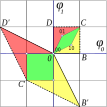
\includegraphics[width=1.0\textwidth]{BernCyc2JacobUnit}
            \end{center}\end{minipage}
            \hspace{2ex}
            \begin{minipage}[c]{0.46\textwidth}
$N_2=3$
\medskip


fixed point ~~$\Xx_{00}$\\
2-cycle ~~~~~~~$\Xx_{01}$, $\Xx_{10}$
            \end{minipage}
\end{center}
    \end{block}
\medskip

square $[0BCD]$
$\Rightarrow\jMorb\Rightarrow$
{\fundPip} $[0B'C'D']$
\end{frame} %%%%%%%%%%%%%%%%%%%%%%%%%%%%%%%%%%%%%%%%%%%%%%

\begin{frame}{fundamental fact for any $\cl{}$}

    \begin{block}{an $\cl{}=3$ example} %{\templatt\ $\cl{}=3$ example}
$\jMorb\,$[unit hyper-cube] = [{\fundPip}]
\begin{center}
            \begin{minipage}[c]{0.32\textwidth}\begin{center}
% ChaosBook {fig:BernPartExam} % BernCyc2Jacob.svg
\includegraphics[width=1.0\textwidth]{PCLength3Counting}
            \end{center}\end{minipage}
            \hspace{2ex}
            \begin{minipage}[c]{0.46\textwidth}
unit hyper-cube $\Xx\in[0,1)^3$
\bigskip\bigskip

{\footnotesize $n>3$ cannot visualize}
            \end{minipage}
\end{center}
    \end{block}
    {\footnotesize
a periodic point $\Rightarrow$ integer lattice point :
{\color{red}$\bullet$} on a face,
{\color{blue}$\bullet$} in the interior
    }
\end{frame} %%%%%%%%%%%%%%%%%%%%%%%%%%%%%%%%%%%%%%%%%%%%%%

\begin{frame}{(2)}
\vfill
\begin{center}
{\huge orbit stability}
\end{center}
\vfill
\end{frame} %%%%%%%%%%%%%%%%%%%%%%%%%%%%%%%%%%%%%%%%%%%%%%

\begin{frame}{(2) orbit stability vs. temporal stability}
\begin{block}{\jacobianOrb}
\(
\jMorb_{ij} =\frac{\delta F[\Xx]_i}{\delta \ssp_j}
\)
stability under {\color{blue}global} perturbation of the whole orbit

\hfill for \cl{} large, a huge $[d\cl{}\!\times\!d\cl{}]$ matrix
\end{block}
\begin{block}{temporal {\jacobianM}}
\(
\jMps%_\Mm
\)
propagates {\color{blue}initial} perturbation $\cl{}$ time steps

\hfill small $[d\!\times\!d]$ matrix
\end{block}
\vfill

$\jMps$ and $\jMorb$ are related by\footfullcite{Hill86}
\begin{block}{Hill's 1886 remarkable formula}
\[
|\Det\jMorb_\Mm| = |\det(\matId - \jMps_\Mm)|
%\label{catHillform}
\]
\end{block}
$\jMorb$ is {\color{red}huge}, even $\infty$\dmn\ matrix\\
$\jMps$ is {\color{red}tiny}, few degrees of freedom matrix
\end{frame} %%%%%%%%%%%%%%%%%%%%%%%%%%%%%%%%%%%%%%%%%%%%%%

\begin{frame}{field theorist's chaos}
    \begin{block}{definition : chaos is}
expanding ~~~~~~~~~~~{\color{blue}\HillDet s}
~~~~~~~~~~~$\Det\jMorb$

exponential $\sharp$~~~~~~~~{\color{blue}field configurations}
~~~~~~~$N_\cl{}$~~~
    \end{block}

\bigskip
%\hfill
the precise sense in which

a (discretized) {\color{blue}field theory}
is {\color{blue}deterministically chaotic}

\vfill
 {\color{red}\huge note} : there is
 {\color{red}no} `time' in this definition
\end{frame} %%%%%%%%%%%%%%%%%%%%%%%%%%%%%%%%%%%%%%%%%%%%%%

\begin{frame}{}
\vfill
\begin{center}
{\huge \po\ theory}
\end{center}
\vfill
\end{frame} %%%%%%%%%%%%%%%%%%%%%%%%%%%%%%%%%%%%%%%%%%%%%%

\begin{frame}{volume of a \po}
Ozorio de Almeida and Hannay\footfullcite{OzoHan84} 1984 :\\
$\sharp$ of periodic points is related to a \JacobianM\ by
\begin{block}{principle of uniformity}
``periodic points of an ergodic system, counted with their natural
weighting, are uniformly dense in phase space''
\end{block}
\bigskip

where
\begin{block}{`natural weight' of \po\ {\Mm}}
\[
  \frac{1}{|\det(\unit - \jMps_{\Mm})|}
\]
\end{block}
\end{frame} %%%%%%%%%%%%%%%%%%%%%%%%%%%%%%%%%%%%%%%%%%%%%%

\begin{frame}{\po s partition lattice states into neighborhoods}
how come {\color{blue}\HillDet} $\Det\jMorb$ counts periodic points ?
\bigskip

`principle of uniformity' is in \footfullcite{CBgetused}
\begin{block}{\po\ theory}
known as the \HREF{http://chaosbook.org/chapters/ChaosBook.pdf\#section.27.4} {flow
conservation} sum rule  :
\beq
\sum_{{\Mm}} %\ssp_i{\in\mbox{\footnotesize Fix}\map^{\cl{}}}}
    \frac{1}{|\det (\unit - \jMps_{\Mm})|}
    \;=
\sum_{{\Mm}} %{\ssp_i{\in\mbox{\footnotesize Fix}\map^{\cl{}}}}
    \frac{1}{|\Det\jMorb_{\Mm}|}
    =1
% \label{H-OdeA_mapsOrb}
\eeq
    {\footnotesize
sum over periodic points $\Xx_{\Mm}$ of period \cl{}
    }
\end{block}

\statesp\ is divided into

\hfill
{\color{blue}neighborhoods} of periodic points of period $\cl{}$
\end{frame} %%%%%%%%%%%%%%%%%%%%%%%%%%%%%%%%%%%%%%%%%%%%%%

\begin{frame}{\po\ counting}
how come a $\Det\jMorb$ counts periodic points ?
\bigskip

\begin{block}{flow conservation sum rule :}
\[
\sum_{\Xx_\Mm{\in\mbox{\footnotesize Fix}\map^{\cl{}}}}
    \frac{1}{|\Det\jMorb_\Mm|}
    =1
% \label{H-OdeA_mapsOrb}
\]
\end{block}
\medskip

Bernoulli system `natural weighting' is simple :
\medskip

the determinant
$\Det\jMorb_\Mm=\Det\jMorb$ the same for all periodic points, whose
number thus verifies the {\color{blue}fundamental fact}
\[
N_\cl{} = |\Det\jMorb|
\] %ee{detBern0}

\medskip


\vfill
    \begin{block}{the number of Bernoulli periodic lattice states}
\(
N_{\cl{}} = |\Det\jMorb| = s^{\cl{}} - 1
\) %\ee{noPerPtsBm}
~~~~~~~~for any $\cl{}$
    \end{block}
\end{frame} %%%%%%%%%%%%%%%%%%%%%%%%%%%%%%%%%%%%%%%%%%%%%%

\begin{frame}{remember the fundamental fact?}
    \begin{block}{period 2 example}
\begin{center}
            \begin{minipage}[c]{0.32\textwidth}\begin{center}
% ChaosBook {fig:BernPartExam} % BernCyc2Jacob.svg
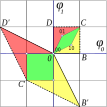
\includegraphics[width=1.0\textwidth]{BernCyc2JacobUnit}
            \end{center}\end{minipage}
            \hspace{2ex}
            \begin{minipage}[c]{0.46\textwidth}
fixed point ~~$\Xx_{00}$\\
2-cycle ~~~~~~~$\Xx_{01}$, $\Xx_{10}$
            \end{minipage}
\end{center}
    \end{block}
\bigskip

$\jMorb\,$[unit hyper-cube] = [{\fundPip}]
\bigskip

look at preimages of the {\fundPip} :
\end{frame} %%%%%%%%%%%%%%%%%%%%%%%%%%%%%%%%%%%%%%%%%%%%%%

\begin{frame}{example : lattice states of period 2}
    \begin{block}{unit hypercube, partitioned}
\begin{center}
            \begin{minipage}[c]{0.32\textwidth}\begin{center}
\includegraphics[width=1.0\textwidth]{BernCyc2JacobPart}
            \end{center}\end{minipage}
            \hspace{2ex}
            \begin{minipage}[c]{0.46\textwidth}
fixed point ~~$\Xx_{00}$\\
2-cycle ~~~~~~~$\Xx_{01}$, $\Xx_{10}$
            \end{minipage}
\end{center}
    \end{block}
\medskip

\begin{block}{
\HREF{http://chaosbook.org/chapters/ChaosBook.pdf\#section.27.4} {flow
conservation} sum rule
            }
\beq
      \frac{1}{|\Det{\color{green}\jMorb_{00}}|}
   +    \frac{1}{|\Det{\color{red}\jMorb_{01}}|}
   + \frac{1}{|\Det{\color{yellow}\jMorb_{10}}|}
    =1
% \label{H-OdeA_mapsOrb}
\eeq
    {\footnotesize
sum over periodic points $\Xx_{\Mm}$ of period $\cl{}=2$
    }
\end{block}

\statesp\ is divided into

\hfill
{\color{blue}neighborhoods} of periodic points of period $\cl{}$
\end{frame} %%%%%%%%%%%%%%%%%%%%%%%%%%%%%%%%%%%%%%%%%%%%%%

%%%%%%%%%%%%%%%%%%%%%%%%%%%%%%%%%%%%%%%%%%%%%%%%%%%%%%%%%%
\begin{frame}{}
\begin{center}
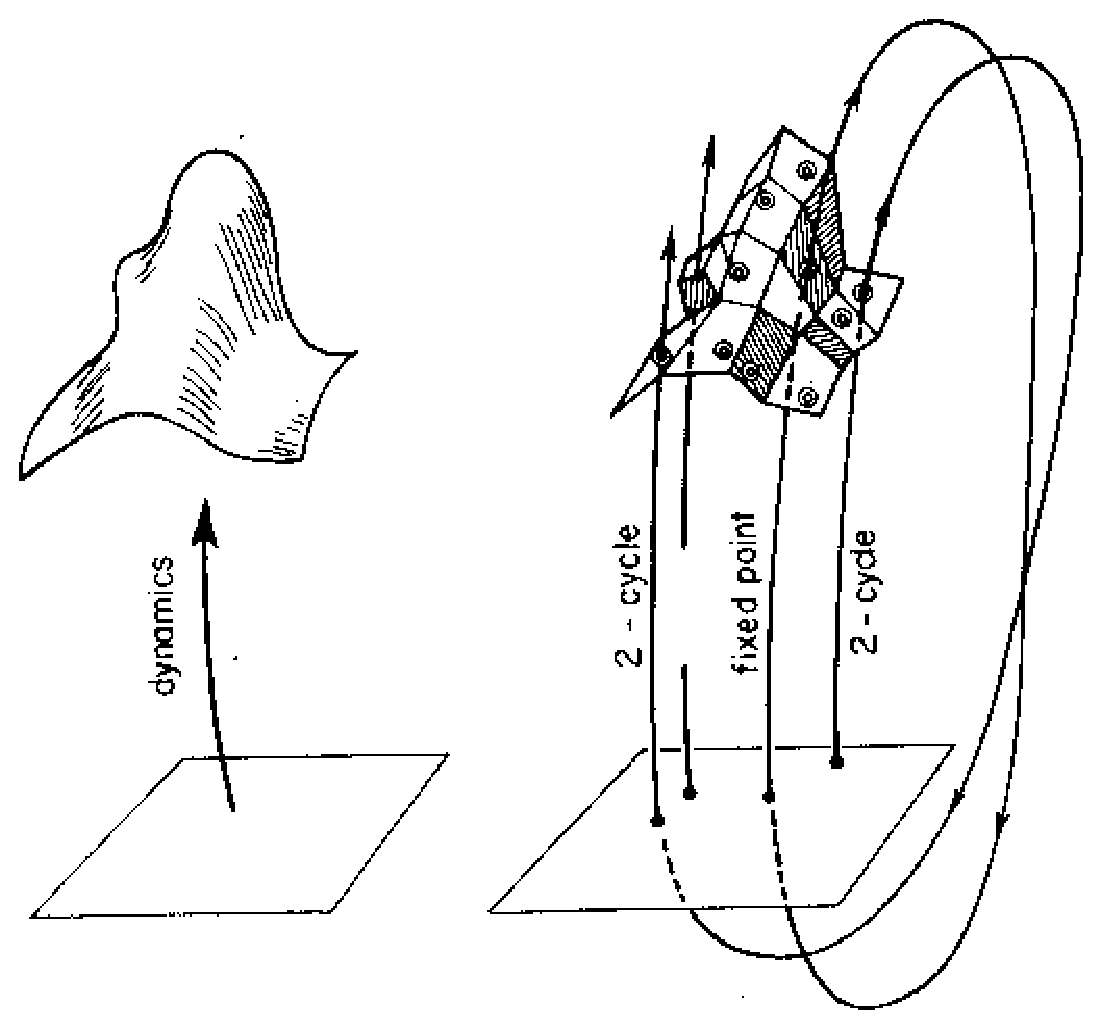
\includegraphics[width=0.60\textwidth]{f_1_08_1}
\end{center}
 tessellate the \statesp\ by {\Large recurrent flows}
\end{frame} %%%%%%%%%%%%%%%%%%%%%%%%%%%%%%%%%%%%%%%%%%%%%%

\begin{frame}{}
\begin{center}
{\huge zeta function}
\end{center}
\vfill
\end{frame} %%%%%%%%%%%%%%%%%%%%%%%%%%%%%%%%%%%%%%%%%%%%%%

\begin{frame}{\po\ theory : counting {\lattstate}s}

\begin{block}{topological zeta function}
\[
\zetatop(z)
 \,=\,  \exp \left(-\sum_{\cl{}=1}^\infty
\frac{z^\cl{}}{\cl{}} N_\cl{}
         \right)
\] %label{BernZeta}
\end{block}
        \begin{enumerate}
              \item
weight ${1}/{\cl{}}$
as by (cyclic) translation invariance, $\cl{}$ {\lattstate}s are
equivalent
              \item
zeta function counts {\color{blue} orbits}, one per each set of equivalent
{\lattstate}s
            \end{enumerate}
\end{frame} %%%%%%%%%%%%%%%%%%%%%%%%%%%%%%%%%%%%%%%%%%%%%%

\begin{frame}{Bernoulli \tzeta}
counts {\color{blue} orbits},
one per each set of {\lattstate}s $N_\cl{}=s^{\cl{}} - 1$
\[
\zetatop(z)
 \,=\,  \exp \left(-\sum_{\cl{}=1}^\infty
\frac{z^\cl{}}{\cl{}} N_n
         \right)
\,=\,
\frac{1 -  {s}z}{1 - z}
\] %label{BernZeta}
numerator $(1 - {s}z)$ says that Bernoulli orbits are built from \\
$s$
fundamental {\color{blue}primitive} {\lattstate}s,

\hfill
the fixed points
$\{\ssp_0,\ssp_1,\cdots,\ssp_{s-1}\}$
\medskip

every other {\lattstate} is
built from their concatenations and repeats.

\vfill
\hfill {\Huge \textcolor{red}{solved!}}
\vfill

{\color{blue}this is `\po\ theory'}
\\
 And if you don't know,
\HREF{https://www.youtube.com/watch?v=_JZom_gVfuw}
{\underline{now you know}}
\end{frame} %%%%%%%%%%%%%%%%%%%%%%%%%%%%%%%%%%%%%%%%%%%%%%

\begin{frame}{summary : think globally, act locally}
\bigskip
the problem of enumerating and determining all {\color{blue}{\lattstate}s}
stripped to its essentials :
\bigskip
\begin{enumerate}
              \item
each solution is a zero of the global {\color{blue}fixed point} condition
\[
F[\Xx] = 0
\]
              \item
{\color{blue}global stability} :  the {\jacobianOrb}
\[
\jMorb_{ij} =\frac{\delta F[\Xx]_i}{\delta \ssp_j}
\]
              \item
{\color{blue}fundamental fact} : the number of period-$\cl{}$ orbits
\[
N_\cl{} = |\Det\jMorb|
\]

              \item
{\color{blue}zeta function} $\zetatop(z)$ : all predictions of the theory
            \end{enumerate}
\end{frame} %%%%%%%%%%%%%%%%%%%%%%%%%%%%%%%%%%%%%%%%%%%%%%

\begin{frame}{next : a kicked rotor} % - templatt.tex }
\begin{bartlett}{
Du mu{\ss}t es dreimal sagen!
        }
\bauthor{
Mephistopheles
    }
\end{bartlett}
\vfill
\begin{enumerate}
              \item \textcolor{gray}{\small
\HREF{http://ChaosBook.org/overheads/spatiotemporal/why.pdf}
{what this is about}
              \item
\HREF{http://ChaosBook.org/overheads/spatiotemporal/Bernoulli.pdf}
{coin toss}
                  }
              \item {\Large
\HREF{http://ChaosBook.org/overheads/spatiotemporal/templatt.pdf}
{kicked rotor}
                  }\textcolor{gray}{\small
              \item
\HREF{http://ChaosBook.org/overheads/spatiotemporal/catlatt.pdf}
{\catlatt}
              \item
\HREF{http://ChaosBook.org/overheads/spatiotemporal/timeDead.pdf}
{bye bye, dynamics}
                    }
            \end{enumerate}
\end{frame} %%%%%%%%%%%%%%%%%%%%%%%%%%%%%%%%%%%%%%%%%%%%%%

%%%%%%%%%%%%%%%%%%%%%%%%%%%%%%%%%%%%%%%%%%%%%%%%%%%%%%%%%%%%%%%%%%%
%%%%%%%%%%%%%%%%%%%%%%%%%%%%%%%%%%%%%%%%%%%%%%%%%%%%%%%%%%%%%%%%%%%
% siminos/presentations/kittens/templatt.tex
\section[a kicked rotor]
 {a kicked rotor}

\begin{frame}{coin toss ? that's not physics !}
Field Theory should be
Hamiltonian and energy conserving \\
Quantum Mechanics requires it

\hfill
because {\color{blue}that is physics} {\color{red}!}
\bigskip

need a system as simple
as the Bernoulli, but {\color{blue}mechanical}
\bigskip

so, we move on from running in circles,

\hfill
to a mechanical {\color{blue}rotor} to kick.
\end{frame} %%%%%%%%%%%%%%%%%%%%%%%%%%%%%%%%%%%%%%%%%%%%%%

\begin{frame}{(1) the traditional cat}
\vfill

\begin{center}
{\huge time-evolution formulation}
% {\huge Hamiltonian formulation}
\end{center}

\vfill
\end{frame} %%%%%%%%%%%%%%%%%%%%%%%%%%%%%%%%%%%%%%%%%%%%%%

\renewcommand{\statesp}{phase space}

\begin{frame}{example of a ``small domain'' dynamics : a single kicked rotor}
an electron circling an atom, subject to

a discrete time
sequence of angle-dependent kicks $F(x_{t})$

\hfill  \includegraphics[width=0.33\textwidth]{kicked-rotor}

\begin{block}{Taylor, Chirikov and Greene  standard map}
\bea
x_{t+1} - x_{t} &=& p_{t+1} \qquad  \mod 1 \continue
p_{t+1} - p_{t} &=& F(x_{t})             \nnu
\eea
\end{block}

\medskip

\hfill $\to$ {\color{red}
chaos in Hamiltonian systems}
\end{frame} %%%%%%%%%%%%%%%%%%%%%%%%%%%%%%%%%%%%%%%%%%%%%%

\begin{frame}{the simplest example : a cat map evolving in time}

force
\(
 F(x) = Kx
\)
{\color{blue}linear} in the displacement $x$
\,,\;
$K\in\integers$
\bea
x_{t+1} &=& x_{t}+p_{t+1} \quad\;\;  \mod 1
        \continue
p_{t+1} &=& p_{t} + K x_{t} \qquad  \textcolor{red}{\mod 1}
\nnu
\eea
 \textcolor{red}{C}ontinuous
 \textcolor{red}{A}utomorphism of the
 \textcolor{red}{T}orus, or

\begin{block}{time-evolution cat map}
a linear, area preserving map of a 2-torus onto itself
 \[
 \left[\begin{array}{c}
   \ssp_{\zeit}  \\
   \ssp_{\zeit+1}
  \end{array} \right]=
  \jMps \left[\begin{array}{c}
   \ssp_{\zeit-1}  \\
   \ssp_{\zeit}
  \end{array} \right]
 - \left[\begin{array}{c}
 0  \\
 \Ssym{\zeit}
 \end{array} \right]
\,,\qquad
\jMps = \left[
\begin{array}{cc}
0 & 1 \\
-1 & s \\
\end{array}
    \right]
 \] %\ee{PerViv:2confRepMat}

\end{block}
for integer {\color{blue}`stretching' $s=\tr{\jMps} > 2$}
the map is \\ beloved by ergodicists :\\
hyperbolic $\Rightarrow$
{\color{blue}perfect chaotic Hamiltonian dynamical system}
\end{frame} %%%%%%%%%%%%%%%%%%%%%%%%%%%%%%%%%%%%%%%%%%%%%%

\begin{frame}{a cat is literally Hooke's wild, `anti-harmonic' sister}

\begin{block}{for $s<2$ Hooke rules}
local restoring oscillations

around the sleepy z-z-z-zzz resting state
\end{block}

\begin{block}{for $s>2$ cats rule}
exponential runaway

wrapped global around a \statesp\ torus
\end{block}
\bigskip

\hfill
{\color{red}cat} is to {\color{red}chaos}
what {\color{red}harmonic oscillator} is to {\color{red}order}
\vfill
\hfill
{\color{blue}there is no more fundamental example of chaos in mechanics}
\end{frame} %%%%%%%%%%%%%%%%%%%%%%%%%%%%%%%%%%%%%%%%%%%%%%

\begin{frame}{(2) {\color{orange}spatio}{\templatt}}
\vfill
\begin{center}
{\huge lattice formulation}
% {\huge Lagrangian formulation}
\end{center}
\vfill
\end{frame} %%%%%%%%%%%%%%%%%%%%%%%%%%%%%%%%%%%%%%%%%%%%%%

\begin{frame}{cat map in lattice formulation}
replace momentum by velocity
\[
p_{t+1}=(\ssp_{t+1}  - \ssp_{t})/\Delta t
\]
obtain
 \[
 \left[\begin{array}{c}
   \ssp_{\zeit}  \\
   {\color{blue}\ssp_{\zeit+1}}
  \end{array} \right]=
  \left[
\begin{array}{cc}
0 & 1 \\
{\color{blue}-1} & {\color{blue}s} \\
\end{array}
    \right]
    \left[\begin{array}{c}
   {\color{blue}\ssp_{\zeit-1}}  \\
   {\color{blue}\ssp_{\zeit}}
  \end{array} \right]
 - \left[\begin{array}{c}
 0  \\
 {\color{blue}\Ssym{\zeit}}
 \end{array} \right]
 \] %\ee{PerViv:2confRepMat}

temporal lattice formulation % $(\ssp_{t},\ssp_{t-1})$
is {\Large pretty}\footfullcite{PerViv} :
\begin{block}{2-step difference equation}
\[
- \ssp_{t+1}  +  s \, \ssp_{t} - \ssp_{t-1} = \Ssym{t}
\] %\ee{eq:CatMapNewton1}
\end{block}
integer $\Ssym{t}$ ensures that

\hfill $\ssp_{t}$ lands in the unit interval

\bigskip
\[
\Ssym{t}\in  \A
\,,\quad \A\ = \{\mbox{finite alphabet}\}
\]
\end{frame} %%%%%%%%%%%%%%%%%%%%%%%%%%%%%%%%%%%%%%%%%%%%%%

\begin{frame}{think globally, act locally}

{\color{orange}spatio}{\templatt} at every instant $\zeit$,
{\color{blue}local} in time
\[
- \ssp_{t+1}  +  s \, \ssp_{t} - \ssp_{t-1} = \Ssym{t}
\] %\ee{eq:CatMapNewton1}
is enforced by the {\color{blue}global} equation
\beq
 \jMorb\,\Xx = \Mm
\,,
\ee{catTempLatt}
where
\end{frame} %%%%%%%%%%%%%%%%%%%%%%%%%%%%%%%%%%%%%%%%%%%%%%

\begin{frame}{orbit Jacobian matrix}
\[
 \jMorb\,\Xx - \Mm= 0
\]
with
\beq
{\Xx} % = \{\ssp_j\}
             = (\ssp_{\zeit+1},\cdots,\ssp_{\zeit+\cl{}})
\,,\quad
{\Mm} % = \{\Ssym{j}\}
             = (\Ssym{{\zeit+1}},\cdots,\Ssym{{\zeit+\cl{}}})
\ee{pathBern}
a
{\color{blue}{\lattstate}}, and a {\color{blue}symbol \brick}
\bigskip

and $[\cl{}\!\times\!\cl{}]$
 {\color{blue}\jacobianOrb} \jMorb\ is
\beq
- \shift{} + s\id - \shift{}^{-1}
=  \left(\begin{array}{ccccc}
    {s}   & -1    &      &         & -1\cr
    -1    & {s}   &-1    &         &   \cr
          & -1    &      & \ddots  &   \cr
          &       &      & {s}     &-1 \cr
    -1    &       &      & -1      & {s}
          \end{array} \right)
\ee{hopMatrix}
\end{frame} %%%%%%%%%%%%%%%%%%%%%%%%%%%%%%%%%%%%%%%%%%%%%%

\begin{frame}{think globally, act locally}
solving the {\color{orange}spatio}{\templatt} equation
\[
\jMorb\Xx=\Mm
\,,
\]
with
the $[\cl{}\!\times\!\cl{}]$ matrix ~~~~~
\(
\jMorb = -\shift{} + s\id - \shift{}^{-1}
\) %{tempBernFix}
\medskip

can be viewed as a search for zeros of the function
\beq
F[\Xx] = \jMorb\Xx-\Mm = 0
\ee{tempFixPoint}
where the entire {\color{blue}global lattice state} ${\Xx}_{\Mm}$ is
\medskip

a single {\color{blue}fixed point}
${\Xx}_{\Mm}=(\ssp_1,\ssp_{2},\cdots,\ssp_{\cl{}})$

\hfill\includegraphics[width=0.12\textwidth]{hyperCube}

\hfill
in the \cl{}\dmn\ unit hyper-cube ~~~~~~~~~~~$\Xx\in[0,1)^\cl{}$
\end{frame} %%%%%%%%%%%%%%%%%%%%%%%%%%%%%%%%%%%%%%%%%%%%%%

\begin{frame}{fundamental fact in action}
% BernCyc2Jacob.svg
    \begin{block}{\templatt\  {\fundPip} for period 2}
square $[0BCD]$
$\Rightarrow\jMorb\,=\,$
{\fundPip} $[0B'C'D']$
\bigskip

\begin{center}
            \begin{minipage}[c]{0.32\textwidth}\begin{center}
% ChaosBook {fig:BernPartExam}
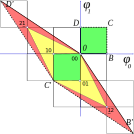
\includegraphics[width=1.0\textwidth]{catCyc2JacobUnit}
            \end{center}\end{minipage}
            \hspace{2ex}
            \begin{minipage}[c]{0.46\textwidth}
$N_2=|\Det\jMorb|=5$
\medskip

{\fundPip} \\
$=$  5 unit area quadrilaterals
            \end{minipage}
\end{center}
a periodic point per each unit volume
    \end{block}
\end{frame} %%%%%%%%%%%%%%%%%%%%%%%%%%%%%%%%%%%%%%%%%%%%%%

\begin{frame}{{\color{orange}spatio}{\templatt}  zeta function}
is the generating function that counts {\color{blue}orbits}
\medskip

substituting the {\color{blue}\HillDet} count of periodic lattice states
\[
N_n = \Det\jMorb
\]
into the
{topological} zeta func\-tion
\[
\zetatop(z)
  =   \exp \left(
    -\sum_{n=1} \frac{z^n}{n} N_n
    \right)
\]%\label{perOrbits:Isola90-13}
leads to the elegant explicit formula\footfullcite{Isola90}
\[
\zetatop(z)
 =  \frac{1 - s z + z^2}
         {1 - 2z + z^2}
\]%\label{perOrbits:Isola90-13}


\vfill\hfill
{\Huge \textcolor{red}{solved!}}
\end{frame} %%%%%%%%%%%%%%%%%%%%%%%%%%%%%%%%%%%%%%%%%%%%%%

\begin{frame}{what continuum theory is \templatt\ discretization of?}
have
\begin{block}{2-step difference equation}
\[
- \ssp_{t+1} + s \, \ssp_{t} - \ssp_{t-1}
    =
\Ssym{t}
\] %\ee{eq:CatMapNewton1}
\end{block}
discrete lattice
\begin{block}{Laplacian in $1$ dimension}
\[
\ssp_{t+1} - 2\ssp_{t} + \ssp_{t-1}
     =
\Box\,\ssp_t
\]
\end{block}
\medskip

so \templatt\ is an (anti)oscillator chain, known as
\begin{block}{$d=1$ Klein-Gordon (or damped Poisson) equation (!)}
\[
 (-\Box + {\mu}^2)\,\ssp_{t} = \m_t
\,, \qquad
{\mu}^2= s-2
\] %\ee{LinearConn}
\end{block}
\vfill\hfill
\textcolor{red}{did you know that a cat map can be so cool?}
\end{frame} %%%%%%%%%%%%%%%%%%%%%%%%%%%%%%%%%%%%%%%%%%%%%%

\begin{frame}{that's it! for spacetime of {\color{blue}any} dimension}
lattice Klein-Gordon equation
    {\Huge
\[
  (-\Box + {\mu}^2)\,\ssp_{t} = \m_t
%    \,, \qquad
\] %\ee{LinearConn}
    }
\hfill solved completely and analytically!
\end{frame} %%%%%%%%%%%%%%%%%%%%%%%%%%%%%%%%%%%%%%%%%%%%%%


\begin{frame}{summary : think globally, act locally}
\bigskip
the problem of determining all global solutions stripped
to its bare essentials :
\bigskip
\begin{enumerate}
              \item
each solution a zero of the global {\color{blue}fixed point} condition
\[
F[\Xx] = 0
\]
              \item
compute  the {\jacobianOrb}
\[
\jMorb_{ij} =\frac{\delta F[\Xx]_i}{\delta \ssp_j}
\]
              \item
{\color{blue}fundamental fact} ~~~~~~~~
\(
N_\cl{} = |\Det\jMorb| =
\)
 period-$\cl{}$ states

 \bigskip
              \item
\hfill $\Rightarrow$ {\color{blue}zeta function} $\zetatop(z)$
            \end{enumerate}
\end{frame} %%%%%%%%%%%%%%%%%%%%%%%%%%%%%%%%%%%%%%%%%%%%%%




%%%%%%%%%%%%%%%%%%%%%%%%%%%%%%%%%%%%%%%%%%%%%%%%%%%%%%%%%%%%%%%%%%%
%%%%%%%%%%%%%%%%%%%%%%%%%%%%%%%%%%%%%%%%%%%%%%%%%%%%%%%%%%%%%%%%%%%
\section[time reversal]
 {time reversal}
\label{s:refersal}

% siminos/presentations/kittens/reversal.tex        pdflatex reversal; biber reversal

%\section[what this talk is about]
% {what this talk is about}
%
%\begin{frame}{overview}
%\begin{enumerate}
%              \item {\Large
%what this is about
%                  }\textcolor{gray}{\small
%%\\{\scriptsize \em
%%  (to skip the motivational blah blah: go to part \textcolor{red}{\ref{spacetimeFT}})
%%  }
%              \item
%chaos - a short course
%              \item
%\templatt
%              \item
%\catlatt
%              \item
%space is time
%              \item
%bye bye, dynamics
%                    }
%            \end{enumerate}
%\end{frame} %%%%%%%%%%%%%%%%%%%%%%%%%%%%%%%%%%%%%%%%%%%%%%

\begin{frame}{}
\vfill
\begin{center}
{\huge chaotic field theory}
\end{center}
\vfill
\end{frame} %%%%%%%%%%%%%%%%%%%%%%%%%%%%%%%%%%%%%%%%%%%%%%

\begin{frame}{Euclidean lattice field theory}
    \begin{block}{scalar \emph{field} $\ssp(x)$}
 evaluated on lattice points
%\bigskip

\begin{center}
            \begin{minipage}[c]{0.32\textwidth}\begin{center}
\includegraphics[width=0.95\textwidth]{MunWal00lattice}
            \end{center}
% 3$d$ lattice
% \label{fig:MunWal00lattice}
            \end{minipage}
            \hspace{2ex}
            \begin{minipage}[c]{0.46\textwidth}
$\ssp_z
=
\ssp(x)$
\\
$
x = a\,z= \mbox{lattice point}$
\\
$
z \in \integers^d %/\speriod{}^d
$
%\ee{LattField}
            \end{minipage}
\end{center}
a periodic point per each unit cell
    \end{block}
\footfullcite{MunWal00}
\end{frame} %%%%%%%%%%%%%%%%%%%%%%%%%%%%%%%%%%%%%%%%%%%%%%

\begin{frame}{example : discretization of a $1d$ field}
    \begin{block}{scalar \emph{field} $\ssp(x)$ evaluated on lattice points}

\begin{center}
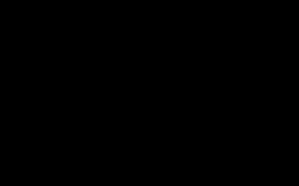
\includegraphics[width=0.55\textwidth]{LC21FieldConfig}

\bigskip
            \begin{minipage}[c]{0.42\textwidth}
periodic field $\ssp(\zeit)$
\\
is a function of
\\
continuous coordinate $\zeit$
            \end{minipage}
            \hspace{2ex}
            \begin{minipage}[c]{0.42\textwidth}
corresponding discretized period-$5$ {\lattstate}
\\
$\Xx=\cycle{\ssp_0 \ssp_1 \ssp_2 \ssp_3 \ssp_4}$,
            \end{minipage}
\end{center}
    \end{block}
Horizontal: $\zeit$ coordinate, lattice sites marked by
\\
dots, labelled by $\zeit\in\integers$

\medskip
the value of the discretized field $\ssp_\zeit\in\reals$ is plotted as
\\
a bar centred at lattice site $\zeit$
\end{frame} %%%%%%%%%%%%%%%%%%%%%%%%%%%%%%%%%%%%%%%%%%%%%%

\begin{frame}{Bravais cell lattice tiling}
 write a periodic field over \cl{}-sites Bravais cell as \\
the {\color{blue}{\lattstate}} and
the {\color{blue}symbol \brick} (sources)
\beq
{\Xx} % = \{\ssp_j\}
             = (\ssp_{\zeit+1},\cdots,\ssp_{\zeit+\cl{}})
\,,\quad
{\Mm} % = \{\Ssym{j}\}
             = (\Ssym{{\zeit+1}},\cdots,\Ssym{{\zeit+\cl{}}})
\ee{pathBern}
\begin{center}
\includegraphics[width=0.85\textheight]{HL1dLatticeStateBar1}
\end{center}

`$\Mm$' for `marching orders' ~~:~~ come here, then go there, $\cdots$
\end{frame} %%%%%%%%%%%%%%%%%%%%%%%%%%%%%%%%%%%%%%%%%%%%%%

\begin{frame}{field theory is defined by its action}
    \begin{block}{field theory}
\textcolor{blue}{field configuration} \Xx\ occurs with probability
\[
p(\Xx)\,=\, \frac{1}{Z}\,e^{-S[\Xx]}
\,,\qquad Z=Z[0]
\] % ee{ProbConf}
\textcolor{blue}{partition function} $=$ sum over all
configurations
\beq
Z[\source]	% = e^{W[\source]}
    \,=\, \int [d\ssp]\,e^{-S[\Xx] + \Xx \cdot \source}
    \,,\qquad
\left[ d\ssp\right] = \prod_{z}^{\lattice} \frac{d\ssp_z}{\sqrt{2 \pi}}
\label{n-pt-corr}
\eeq

\textcolor{blue}{`source'} $\source$
    \end{block}
\end{frame} %%%%%%%%%%%%%%%%%%%%%%%%%%%%%%%%%%%%%%%%%%%%%%

\begin{frame}{example : Euclidean {$\phi^4$} theory}
    \begin{block}{continuum action}
\bea
S &=&
\int dx^d \left\{ \frac{1}{2} \sum_{i =1}^d
(\partial_{\mu}\ssp(x))^2 + \frac{\mu^2}{2}\ssp(x)^2 + \frac{g}{4!}\ssp(x)^4
\right\}
\eea
    \end{block}

    \begin{block}{lattice action}
\bea
S[\Xx] &=&
\sum_{z,z'} \frac{1}{2}\left\{
\ssp_z\left(-\Box + \mu^2\right)_{zz'}\ssp_{z'}
\right\}
 + \sum_{z}\frac{g}{4!}\ssp_z^4
\,.
%\label{MunWal00freeAct}
\eea
    \end{block}

in `lattice units' : \(a=1\)
\end{frame} %%%%%%%%%%%%%%%%%%%%%%%%%%%%%%%%%%%%%%%%%%%%%%

\begin{frame}{QFT path integrals : semi-classical WKB quantization}
  \begin{columns}
  \column{0.42\textwidth}
\begin{block}{WKB backbone}
\textcolor{blue}{classical field theory}
\\
extremal condition $\to$ eqs
\beq
\frac{\delta{S[\Xx]}}{\delta\ssp_z~}=\Ssym{z}
\ee{LC21eqMotion}
classical solution \Xx\ satisfies
the extremal condition on every lattice site
\end{block}
  \column{0.50\textwidth}
\begin{block}{a fractal set of saddles}
\includegraphics[width=1.00\textwidth,clip=true]{pde2}%
\end{block}
  \end{columns}
\end{frame}

\begin{frame}{think globally, act locally}
    \begin{center}
\includegraphics[width=0.85\textwidth]{globalLocal}
    \end{center}
for each symbol array \Mm, a periodic {\lattstate} $\Xx_\Mm$
\end{frame} %%%%%%%%%%%%%%%%%%%%%%%%%%%%%%%%%%%%%%%%%%%%%%

\begin{frame}{orbit Jacobian (Hill, Hessian, ...)  matrix}
each {\lattstate} has its own
\beq
\jMorb[\Xx] =
\left(\begin{array}{cccccccc}
%\begin{pmatrix}
 {s}_{0} &-1 & 0 & 0 & \cdots & 0 & 0 &-1 \\
-1&  {s}_{1} &-1 & 0 & \cdots & 0 & 0 & 0 \\
0 &-1 &  {s}_{2} &-1 & \cdots & 0 & 0 & 0 \\
\vdots & \vdots & \vdots & \vdots & \ddots & \vdots & \vdots & \vdots \\
0 & 0 & 0 & 0 & \cdots &-1 &  {s}_{\cl{}-2} &-1 \\
-1& 0 & 0 & 0 & \cdots & 0 &-1 &  {s}_{\cl{}-1}
%\end{pmatrix}
          \end{array} \right)
\,,
\ee{jMorb1dFT} %was {jMorb1dField}, {PCJiKoKr20(8)}
{\color{orange}stretching factor} ${s}_{\zeit}= V''[\ssp_{\zeit}]$ is
\\
function of the site field $\ssp_\zeit$ for the
given \lattstate\ $\Xx$

\bigskip
  \begin{enumerate}
              \item
can compute {\color{blue}\HillDet} $\Det\jMorb$
              \item
Hill-Lindstedt-Poincar\'e : \\
all calculations should be done
on reciprocal lattice
              \item
toolbox : discrete Fourier transforms, irreps of \Dn{n}
   \end{enumerate}
\end{frame} %%%%%%%%%%%%%%%%%%%%%%%%%%%%%%%%%%%%%%%%%%%%%%

\begin{frame}{popular 1$d$ lattice field theories}

{\color{orange}spatio}temporal lattice field theory
\bea
- \ssp_{\zeit+1}  + V'[\ssp_{\zeit}] - \ssp_{\zeit-1}
    &=&
\Ssym{\zeit}
%\,,\qquad  \ssp_{\zeit} \in [0,1)
%\label{LC21:1dTempFT}
\eea

{\color{orange}spatio}temporal  Bernoulli
\bea
- \ssp_{\zeit+1} + {s}\,\ssp_{\zeit}
    \qquad\quad\;
    &=&
\Ssym{\zeit}
%\,,\qquad  \ssp_{\zeit} \in [0,1)\,,
%\label{LC21:1dBernLatt}    % labelled {1stepDiffEq} elsewhere
\eea

{\color{orange}spatio}{\templatt}
\bea
- \ssp_{\zeit+1}  +  \,{s}\,\ssp_{\zeit} - \ssp_{\zeit-1}
    &=&
\Ssym{\zeit}
%\,,\qquad  \ssp_{\zeit} \in [0,1)
\eea %    \continue %\label{LC21:1dTemplatt}\\
{\color{orange}spatio}{\henlatt}
\bea
- \ssp_{\zeit+1} + {a}\,\ssp_{\zeit}^2 - \ssp_{\zeit-1}
    &=&
\Ssym{\zeit}
%\,,\qquad  \Ssym{\zeit}=2
\eea %    \continue %\label{LC21:1dHenlatt}\\
{\color{orange}spatio}temporal {$\phi^4$} theory
\bea
- \ssp_{\zeit+1} + \frac{g}{3!}\ssp_{\zeit}^3 - \ssp_{\zeit-1}
    &=&
\Ssym{\zeit}
%\,,
%\label{LC21:1dPhi4}
\eea
\end{frame} %%%%%%%%%%%%%%%%%%%%%%%%%%%%%%%%%%%%%%%%%%%%%%

\begin{frame} {in crystallography symmetries rule}
There are only two \HREF{https://en.wikipedia.org/wiki/Line_group}
{1\dmn\ space groups}  $\Group$:
\\
\textcolor{blue}{$p1$} \emph{infinite cyclic
group}  \Cn{\infty} of all lattice translations,
\beq
\Cn{\infty}
    =       \{
\cdots, \shift{-2}, \shift{-1},
        1,
        \shift{1}, \shift{2}, \shift{3}, \cdots
             \}
\label{C_infty}
\eeq

\textcolor{blue}{$p1m$} \emph{infinite dihedral group} $\Dn{\infty}$  of all
translations and reflections\footfullcite{KiLePa03},
\beq
  \Dn{\infty} = \{
\cdots, \shift{-2},\Refl_{-2}, \shift{-1},\Refl_{-1},
        1,\Refl,
        \shift{1},\Refl_{1}, \shift{2},\Refl_{2}, \cdots
             \}
%\,.
\ee{LC21D_infty}
\end{frame} %%%%%%%%%%%%%%%%%%%%%%%%%%%%%%%%%%%%%%%%%%%%%%

\begin{frame} {4 kinds of Bravais lattice states}
\begin{center}
{$(n)$}
\includegraphics[width=0.40\textwidth]{HL1dLatticeStateBar1}\quad~~~
{$(o)$}
\includegraphics[width=0.40\textwidth]{HL1dLatticeStateBar2}
\\ %~~~
{$(ee)$}
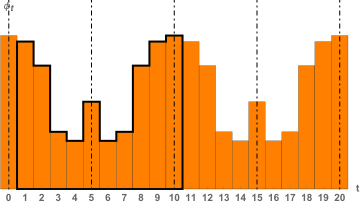
\includegraphics[width=0.40\textwidth]{HL1dLatticeStateBar4}\quad
{$(eo)$}
\includegraphics[width=0.40\textwidth]{HL1dLatticeStateBar3}
%\caption{\label{fig:symmLattStates}
  \end{center}

$(n)$ {\em no reflection symmetry:}
    $H_{5}$ invariant period-5 {\lattstate}

$(o)$ {\em odd period, symmetric:}
    an $H_{9,8}$ invariant period-9

$(ee)$ {\em even period, even symmetric:}
    $H_{10,0}$  invariant period-10

$(eo)$ {\em even period, odd symmetric:}
    $H_{10,9}$  invariant period-10
\end{frame} %%%%%%%%%%%%%%%%%%%%%%%%%%%%%%%%%%%%%%%%%%%%%%

\begin{frame} {group actions}
\textcolor{blue}{group multiplication}
$\LieEl_i\LieEl_j$
\beq
\begin{tabular}{c|cc}
%\Dn{\infty} &\shift{j}        &\Refl_j\\\hline
            &$\shift{j}$        &$\Refl_j$\\\hline
$\shift{i}$  &$\shift{i+j}$     &$\Refl_{j-i}$\\
$\Refl_i$   &$\Refl_{i+j}$     &$\shift{j-i}$
\end{tabular}
\ee{eq:DinftyMultTab}
either adds up translations,
\\
or shifts and then reverses their direction
\end{frame} %%%%%%%%%%%%%%%%%%%%%%%%%%%%%%%%%%%%%%%%%%%%%%

\begin{frame} {$\Dn{\infty}$ orbit of a generic {\lattstate}}
%%%%%%%%%%%%%%%%%%%%%%%%%%%%%%%%%%%%%%%%%%%%%%%%%%%%%
\begin{center}
  \begin{minipage}[b]{0.17\textwidth}\begin{center}
{(1)}~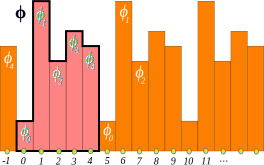
\includegraphics[width=\textwidth]{1dLatStatC_5_0}
\\
{($\shift{1}$)}~\includegraphics[width=\textwidth]{1dLatStatC_5_1}
\\
{($\shift{2}$)}~\includegraphics[width=\textwidth]{1dLatStatC_5_2}
\\
{($\shift{3}$)}~\includegraphics[width=\textwidth]{1dLatStatC_5_3}
\\
{($\shift{4}$)}~\includegraphics[width=\textwidth]{1dLatStatC_5_4}
  \end{center}\end{minipage}
\qquad\quad
  \begin{minipage}[b]{0.17\textwidth}\begin{center}
{($\Refl$)}~\includegraphics[width=\textwidth]{1dLatStatC_5_s0}
\\
{($\Refl_1$)}~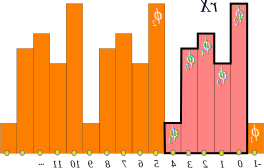
\includegraphics[width=\textwidth]{1dLatStatC_5_s1}
\\
{($\Refl_2$)}~\includegraphics[width=\textwidth]{1dLatStatC_5_s2}
\\
{($\Refl_3$)}~\includegraphics[width=\textwidth]{1dLatStatC_5_s3}
\\
{($\Refl_4$)}~\includegraphics[width=\textwidth]{1dLatStatC_5_s4}

  \end{center} \end{minipage}
  \end{center}
%  \caption{\label{fig:1dLatStatC_5}
% (1)
{\lattstate}
% \refeq{1dLattStatC_n}
\(\Xx=\cycle{\ssp_0 \ssp_1 \ssp_2 \ssp_3 \ssp_4}\),
no reflection symmetry
\\

\Dn{\infty}-orbit is isomorphic to $\Dn{5}$ : $10$ distinct {\lattstate}s
\end{frame} %%%%%%%%%%%%%%%%%%%%%%%%%%%%%%%%%%%%%%%%%%%%%%

\begin{frame} {zeta functions unlike 1980's}

{\po\ theory : counting {\lattstate}s}\footfullcite{Lind96}

\begin{block}{Lind zeta function}
\beq
\zeta_{Lind}(t) =
\exp \left( \sum_{H} \;
            \frac{N_{H}}{|\Group/{H}|}t^{|\Group/H|}
      \right)
\ee{LC21Ryu17eq:1.3}
sum is over all subgroups $H$ of space group $\Group$
\\
$N_{H}$ is the number of fixed points of $H$
\\
$|\Group/{H}|$ is the number of states in $H$ orbit
\end{block}
        \begin{enumerate}
              \item
Lind zeta function counts group {\color{blue} orbits}, one per each set of equivalent
{\lattstate}s
            \end{enumerate}
\end{frame} %%%%%%%%%%%%%%%%%%%%%%%%%%%%%%%%%%%%%%%%%%%%%%

\begin{frame} {zeta functions unlike 1980's}

{\po\ theory :
\\
counting {\lattstate}s} for reflection-symmetric systems%
\footfullcite{ArtMaz65}${}^,$\footfullcite{KiLePa03}

\begin{block}{Kim-Lee-Park zeta function}
\beq
\zeta_{\Refl}(t) = \sqrt{\zeta_{top}(t^2)} \; e^{h(t)},
\ee{LC21Ryu17eq:2.1}
where $\zeta_{top}$ is the
Artin-Mazur zeta function,
and the counts of the 3 kinds of symmetric orbits are
\beq
h(t) = \sum_{m=1}^{\infty} \left\{
       N_{2m-1, 0}\,t^{2m-1}
       + \left(N_{2m,0}+N_{2m,1}\right)\,\frac{ t^{2m}}{2}
                               \right\}
\ee{LC21Ryu17eq:2.11}
\end{block}
\end{frame} %%%%%%%%%%%%%%%%%%%%%%%%%%%%%%%%%%%%%%%%%%%%%%


%%%%%%%%%%%%%%%%%%%%%%%%%%%%%%%%%%%%%%%%%%%%%%%%%%%%%%%%%%%%%%%%%%%
%%%%%%%%%%%%%%%%%%%%%%%%%%%%%%%%%%%%%%%%%%%%%%%%%%%%%%%%%%%%%%%%%%%
% siminos/presentations/kittens/timeDead.tex        pdflatex timeDead; biber timeDead
\section[bye bye, dynamics]
 {bye bye, dynamics}
\label{s:byeDynamics}


\begin{frame}{}
\begin{enumerate}
              \item \textcolor{gray}{\small
%what this is about
%              \item
coin toss
              \item
kicked rotor
              \item
\catlatt
                  }
              \item {\Large
bye bye, dynamics
%                  }\textcolor{gray}{\small
%              \item
%bye bye, dynamics
                    }
            \end{enumerate}
\end{frame} %%%%%%%%%%%%%%%%%%%%%%%%%%%%%%%%%%%%%%%%%%%%%%

\begin{frame}{insight 1 : how is turbulence described?}
\begin{block}{not by the evolution of an initial state}
exponentially unstable system have finite (Lyapunov) time and
space prediction horizons
\end{block}
but
\bigskip

\begin{block}{by enumeration of admissible field configurations}
and their natural weights
\end{block}
\end{frame} %%%%%%%%%%%%%%%%%%%%%%%%%%%%%%%%%%%%%%%%%%%%%%

\begin{frame}{insight 2 : description of turbulence by d-tori}
\begin{block}{1 time, 0 space dimensions}
a {\statesp} point is {\em periodic} if its orbit returns to itself
after a finite time \period{}; such orbit tiles the time axis
by infinitely many repeats
\end{block}

\bigskip

\begin{block}{1 time, $d$-1 space dimensions}
 a {\statesp} point is {\em spatiotemporally periodic} if
it belongs to \\ an invariant $d$-torus ${\R}$,\\
\ie, a \brick\ $\Mm_{\R}$ that
tiles the lattice state  $\Mm$, \\
with period $\ell_j$ in $j$th lattice direction
\end{block}
\end{frame} %%%%%%%%%%%%%%%%%%%%%%%%%%%%%%%%%%%%%%%%%%%%%%

\begin{frame}{insight 3 : can compute `all' solutions}
Bernoulliland - rough initial guesses converge

\bigskip

no exponential instabilities

\bigskip

reciprocal lattice
\end{frame} %%%%%%%%%%%%%%%%%%%%%%%%%%%%%%%%%%%%%%%%%%%%%%

\begin{frame} {what we still do not understand today}
  \begin{enumerate}
              \item
solved so far only 1\dmn\ {\color{orange}spatio}{temporal} lattice,
\\
point group \Dn{1}
              \item
should all time-reversal symmetric systems be analyzed this way ?
              \item
should all dynamical systems should be solved on reciprocal lattice ?
              \item
for 2\dmn\ \spt\ chaotic field theory,
\\
still have to do this for square lattice point group \Dn{4}
              \item
then, solve the problem of turbulence \\
(Navier-Stokes, Yang-Mills, general relativity)
   \end{enumerate}
\end{frame} %%%%%%%%%%%%%%%%%%%%%%%%%%%%%%%%%%%%%%%%%%%%%%

\begin{frame}{Verbrechen des Jahrhunderts : das Ende der Zeit}
\begin{center}
\textcolor{red}{{\huge die Zeit ist tot}
    \\
{also, an die Arbeit!}}
\end{center}
\end{frame} %%%%%%%%%%%%%%%%%%%%%%%%%%%%%%%%%%%%%%%%%%%%%%

\begin{frame}{bye bye, dynamics}
\begin{enumerate}
              \item
goal : describe states of turbulence in infinite spatiatemporal domains
              \item
theory : classify, enuremate all spatiotemporal tilings
              \item
example : \catlatt, the simplest model of ``turbulence''
\end{enumerate}

\vfill

there is no more time

\medskip

there is only enumeration of

\hfill
admissible spacetime field configurations
\end{frame} %%%%%%%%%%%%%%%%%%%%%%%%%%%%%%%%%%%%%%%%%%%%%%

\begin{frame}{crime of the century : this the end of time}
\begin{center}
\textcolor{red}{{\huge time is dead}
    \\
{now, get to work}}
\end{center}
\end{frame} %%%%%%%%%%%%%%%%%%%%%%%%%%%%%%%%%%%%%%%%%%%%%%

\begin{frame}{take-home :   }
\begin{center}
            \begin{minipage}[c]{0.40\textwidth}\begin{center}
traditional field theory
\bigskip

\includegraphics[width=0.85\textwidth]{mattressSpring}\\
{\color{blue}Helmholtz}
            \end{center}\end{minipage}
            \hspace{2ex}
            \begin{minipage}[c]{0.46\textwidth}\begin{center}
chaotic field theory\\
\bigskip
\bigskip
\bigskip

\includegraphics[width=1.0\textwidth]{flagellum1}\\
\bigskip

damped {\color{blue}Poisson},  {\color{blue}Yukawa}
            \end{center}\end{minipage}
\end{center}
\end{frame} %%%%%%%%%%%%%%%%%%%%%%%%%%%%%%%%%%%%%%%%%%%%%%

%%% #######################################
\end{document}
